\documentclass[11pt,a4paper]{article}

% Packages
\usepackage[utf8]{inputenc}
\usepackage[T1]{fontenc}
\usepackage{amsmath,amssymb,amsfonts}
\usepackage{graphicx}
\usepackage{booktabs}
\usepackage{multirow}
\usepackage{array}
\usepackage{xcolor}
\usepackage{tikz}
\usetikzlibrary{shapes.geometric, arrows, positioning, fit, backgrounds, calc}
\usepackage{algorithm}
\usepackage{algpseudocode}
\usepackage{listings}
\usepackage{hyperref}
\usepackage{geometry}
\geometry{margin=1in}

% Colors
\definecolor{taxonomy_s}{RGB}{52, 152, 219}
\definecolor{taxonomy_r}{RGB}{46, 204, 113}
\definecolor{taxonomy_c}{RGB}{231, 76, 60}
\definecolor{taxonomy_m}{RGB}{155, 89, 182}
\definecolor{pipeline}{RGB}{241, 196, 15}
\definecolor{kg}{RGB}{26, 188, 156}

% TikZ Styles
\tikzstyle{module} = [rectangle, rounded corners, minimum width=2.5cm, minimum height=1cm, text centered, draw=black, fill=blue!20]
\tikzstyle{data} = [cylinder, shape border rotate=90, draw, minimum height=1.5cm, minimum width=1.5cm, fill=green!20]
\tikzstyle{process} = [rectangle, minimum width=2cm, minimum height=0.8cm, text centered, draw=black, fill=orange!20]
\tikzstyle{arrow} = [thick,->,>=stealth]

\title{\textbf{BioREASONC-Bench: A Reasoning-Centric Benchmark for Evaluating LLM Causal Reasoning in Biomedicine}\\[0.5em]
\large System Architecture and Methodology}

\author{Computational Biology Research}
\date{\today}

\begin{document}

\maketitle

\begin{abstract}
We present BioREASONC-Bench, a comprehensive benchmark designed to evaluate Large Language Models' (LLMs) causal reasoning capabilities in the biomedical domain. Our benchmark is grounded in the CAUSALdb2 knowledge graph containing 66,057 gene-disease associations with Mendelian Randomization (MR) validation. We introduce a four-taxonomy framework (Structure, Risk, Causal, Mechanism) with five answer formats (Yes/No, Multiple Choice, Short, Long, Reasoning) to systematically assess different aspects of biomedical reasoning. This document details the system architecture, implementation methodology, and benchmark generation pipeline.
\end{abstract}

\tableofcontents
\newpage

%==============================================================================
\section{Introduction}
%==============================================================================

Large Language Models have shown remarkable capabilities in natural language understanding and generation. However, their ability to perform accurate causal reasoning in specialized domains like biomedicine remains understudied. BioREASONC-Bench addresses this gap by providing a rigorous evaluation framework that distinguishes between:

\begin{itemize}
    \item \textbf{Association vs. Causation}: Can the model distinguish GWAS associations from MR-validated causal relationships?
    \item \textbf{Evidence Interpretation}: Can the model correctly interpret risk scores, odds ratios, and p-values?
    \item \textbf{Mechanistic Understanding}: Does the model understand biological pathways and protein interactions?
    \item \textbf{Reasoning Depth}: Can the model provide step-by-step logical reasoning for its conclusions?
\end{itemize}

%==============================================================================
\section{System Architecture}
%==============================================================================

\subsection{High-Level Architecture}

Figure \ref{fig:architecture} presents the overall system architecture of BioREASONC-Bench.

\begin{figure}[htbp]
\centering
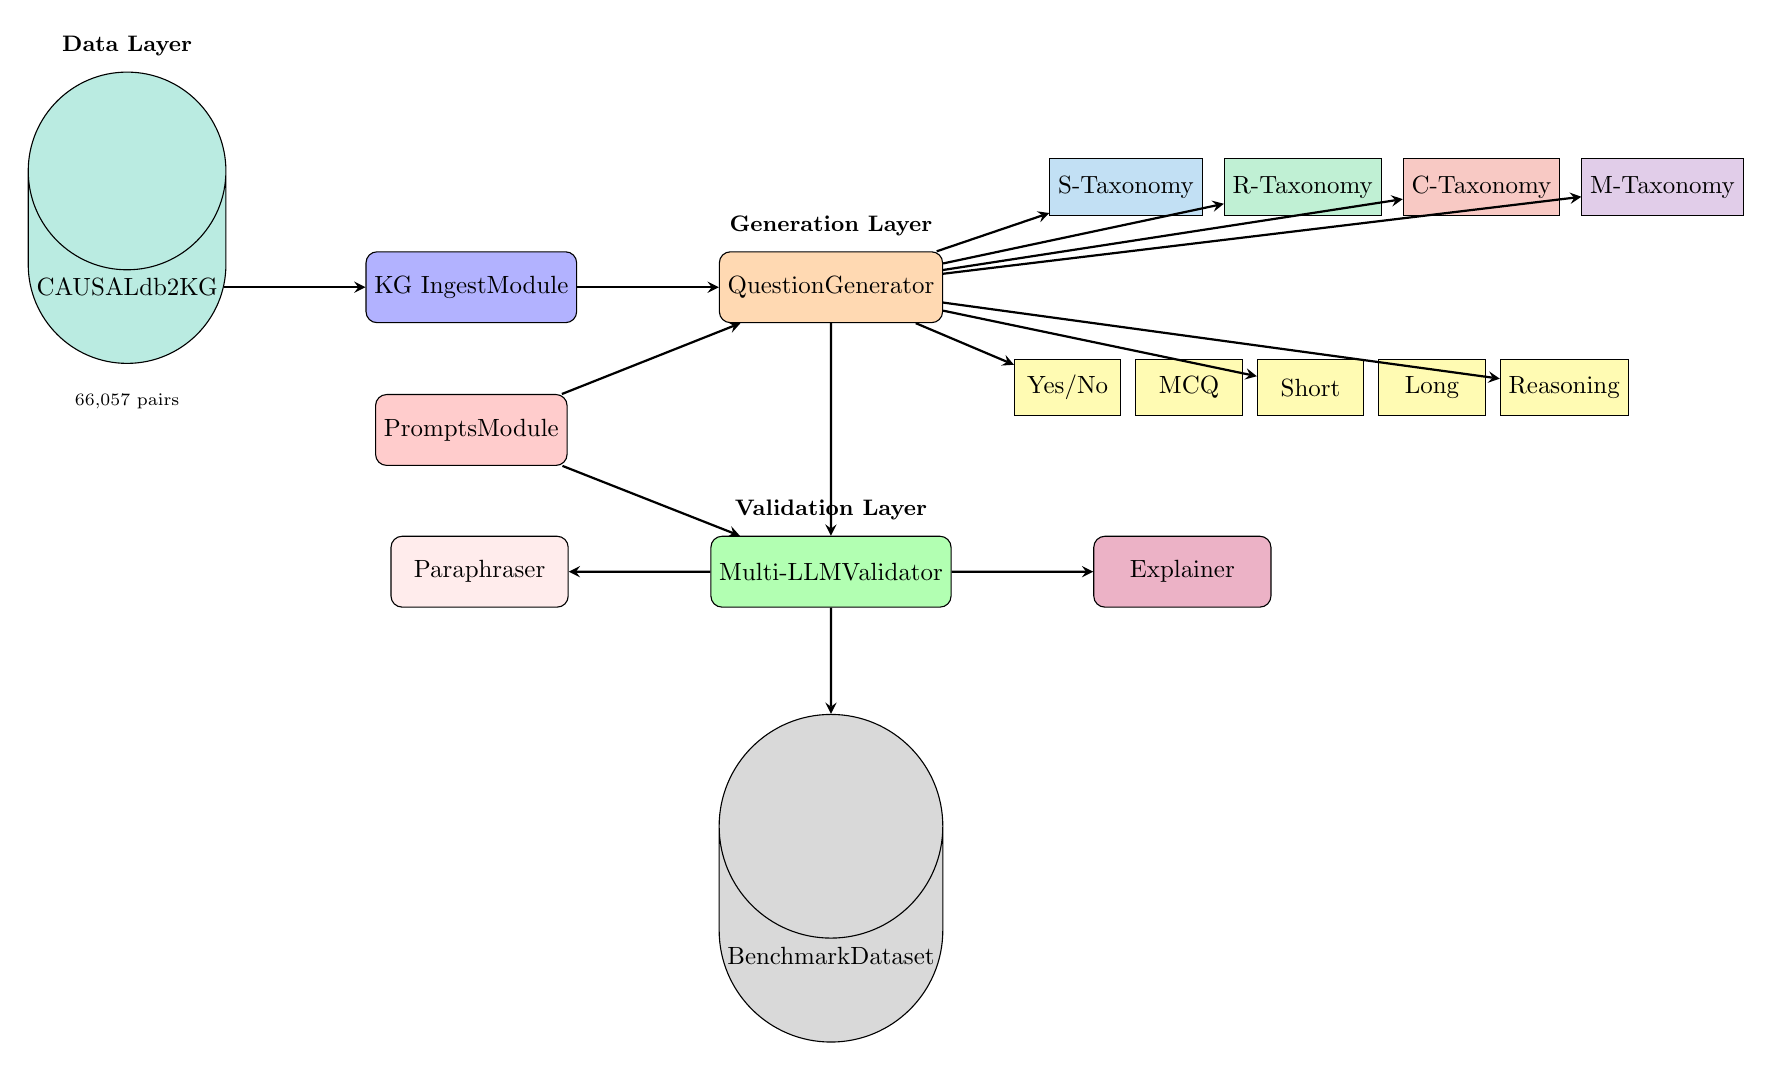
\begin{tikzpicture}[node distance=1.5cm, scale=0.9, transform shape]

% Knowledge Graph Layer
\node[data, fill=kg!30] (kg) {CAUSALdb2\\KG};
\node[below=0.3cm of kg, font=\scriptsize] {66,057 pairs};

% Ingestion Layer
\node[module, right=2cm of kg, fill=blue!30] (ingest) {KG Ingest\\Module};

% Generator Layer
\node[module, right=2cm of ingest, fill=orange!30] (generator) {Question\\Generator};

% Taxonomy boxes
\node[process, above right=0.5cm and 1.5cm of generator, fill=taxonomy_s!30] (tax_s) {S-Taxonomy};
\node[process, right=0.3cm of tax_s, fill=taxonomy_r!30] (tax_r) {R-Taxonomy};
\node[process, right=0.3cm of tax_r, fill=taxonomy_c!30] (tax_c) {C-Taxonomy};
\node[process, right=0.3cm of tax_c, fill=taxonomy_m!30] (tax_m) {M-Taxonomy};

% Format boxes
\node[process, below right=0.5cm and 1cm of generator, fill=yellow!30, minimum width=1.5cm] (fmt1) {Yes/No};
\node[process, right=0.2cm of fmt1, fill=yellow!30, minimum width=1.5cm] (fmt2) {MCQ};
\node[process, right=0.2cm of fmt2, fill=yellow!30, minimum width=1.5cm] (fmt3) {Short};
\node[process, right=0.2cm of fmt3, fill=yellow!30, minimum width=1.5cm] (fmt4) {Long};
\node[process, right=0.2cm of fmt4, fill=yellow!30, minimum width=1.5cm] (fmt5) {Reasoning};

% Validation Layer
\node[module, below=3cm of generator, fill=green!30] (validator) {Multi-LLM\\Validator};

% Explainer
\node[module, right=2cm of validator, fill=purple!30] (explainer) {Explainer};

% Paraphraser
\node[module, left=2cm of validator, fill=pink!30] (paraphraser) {Paraphraser};

% Output
\node[data, below=1.5cm of validator, fill=gray!30] (output) {Benchmark\\Dataset};

% Prompts
\node[module, below=1cm of ingest, fill=red!20] (prompts) {Prompts\\Module};

% Arrows
\draw[arrow] (kg) -- (ingest);
\draw[arrow] (ingest) -- (generator);
\draw[arrow] (generator) -- (tax_s);
\draw[arrow] (generator) -- (tax_r);
\draw[arrow] (generator) -- (tax_c);
\draw[arrow] (generator) -- (tax_m);
\draw[arrow] (generator) -- (fmt1);
\draw[arrow] (generator) -- (fmt3);
\draw[arrow] (generator) -- (fmt5);
\draw[arrow] (generator) -- (validator);
\draw[arrow] (validator) -- (explainer);
\draw[arrow] (validator) -- (paraphraser);
\draw[arrow] (validator) -- (output);
\draw[arrow] (prompts) -- (generator);
\draw[arrow] (prompts) -- (validator);

% Labels
\node[above=0.1cm of kg, font=\small\bfseries] {Data Layer};
\node[above=0.1cm of generator, font=\small\bfseries] {Generation Layer};
\node[above=0.1cm of validator, font=\small\bfseries] {Validation Layer};

\end{tikzpicture}
\caption{BioREASONC-Bench System Architecture}
\label{fig:architecture}
\end{figure}

\subsection{Module Structure}

The system consists of seven core modules organized in a pipeline architecture:

\begin{figure}[htbp]
\centering
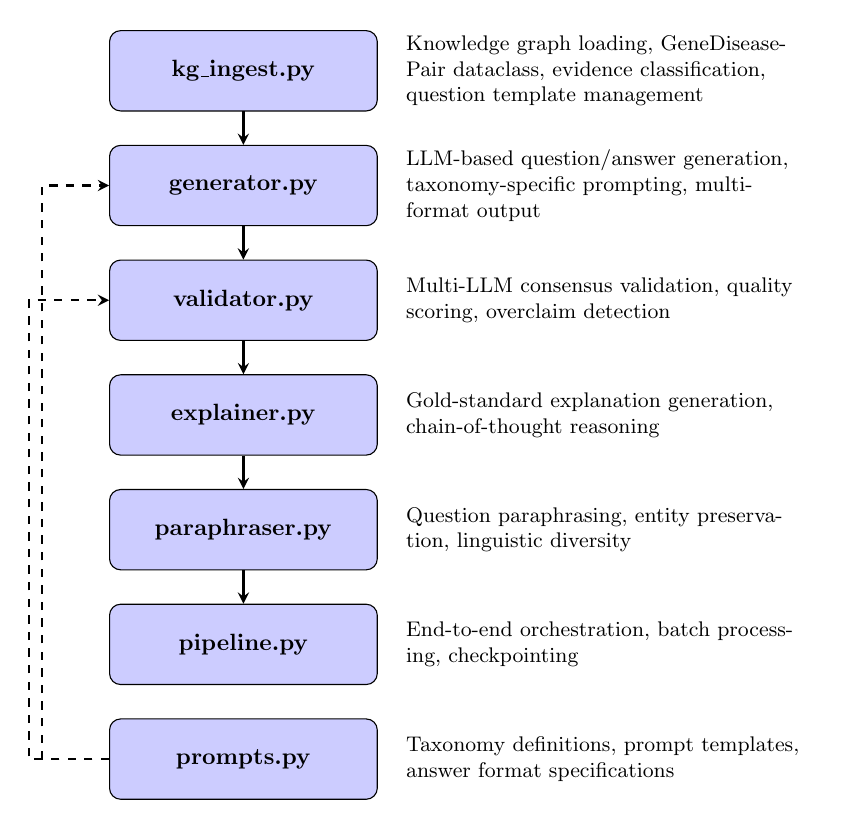
\begin{tikzpicture}[node distance=0.8cm, scale=0.85, transform shape]

% Module boxes with descriptions
\node[module, minimum width=4cm, minimum height=1.2cm] (kg_mod) {
    \textbf{kg\_ingest.py}
};
\node[right=0.3cm of kg_mod, text width=6cm, font=\small] {
    Knowledge graph loading, GeneDiseasePair dataclass, evidence classification, question template management
};

\node[module, minimum width=4cm, minimum height=1.2cm, below=0.5cm of kg_mod] (gen_mod) {
    \textbf{generator.py}
};
\node[right=0.3cm of gen_mod, text width=6cm, font=\small] {
    LLM-based question/answer generation, taxonomy-specific prompting, multi-format output
};

\node[module, minimum width=4cm, minimum height=1.2cm, below=0.5cm of gen_mod] (val_mod) {
    \textbf{validator.py}
};
\node[right=0.3cm of val_mod, text width=6cm, font=\small] {
    Multi-LLM consensus validation, quality scoring, overclaim detection
};

\node[module, minimum width=4cm, minimum height=1.2cm, below=0.5cm of val_mod] (exp_mod) {
    \textbf{explainer.py}
};
\node[right=0.3cm of exp_mod, text width=6cm, font=\small] {
    Gold-standard explanation generation, chain-of-thought reasoning
};

\node[module, minimum width=4cm, minimum height=1.2cm, below=0.5cm of exp_mod] (para_mod) {
    \textbf{paraphraser.py}
};
\node[right=0.3cm of para_mod, text width=6cm, font=\small] {
    Question paraphrasing, entity preservation, linguistic diversity
};

\node[module, minimum width=4cm, minimum height=1.2cm, below=0.5cm of para_mod] (pipe_mod) {
    \textbf{pipeline.py}
};
\node[right=0.3cm of pipe_mod, text width=6cm, font=\small] {
    End-to-end orchestration, batch processing, checkpointing
};

\node[module, minimum width=4cm, minimum height=1.2cm, below=0.5cm of pipe_mod] (prompt_mod) {
    \textbf{prompts.py}
};
\node[right=0.3cm of prompt_mod, text width=6cm, font=\small] {
    Taxonomy definitions, prompt templates, answer format specifications
};

% Arrows connecting modules
\draw[arrow] (kg_mod.south) -- (gen_mod.north);
\draw[arrow] (gen_mod.south) -- (val_mod.north);
\draw[arrow] (val_mod.south) -- (exp_mod.north);
\draw[arrow] (exp_mod.south) -- (para_mod.north);
\draw[arrow] (para_mod.south) -- (pipe_mod.north);
\draw[arrow, dashed] (prompt_mod.west) -- ++(-1,0) |- (gen_mod.west);
\draw[arrow, dashed] (prompt_mod.west) -- ++(-1.2,0) |- (val_mod.west);

\end{tikzpicture}
\caption{Module Structure and Data Flow}
\label{fig:modules}
\end{figure}

%==============================================================================
\section{Methodology}
%==============================================================================

\subsection{Knowledge Graph Foundation}

BioREASONC-Bench is grounded in CAUSALdb2 \cite{causaldb2}, a comprehensive knowledge graph of gene-disease associations derived from genome-wide association studies (GWAS) with Mendelian Randomization validation.

\subsubsection{Data Source Characteristics}

\begin{table}[htbp]
\centering
\caption{CAUSALdb2 Knowledge Graph Statistics}
\label{tab:kg_stats}
\begin{tabular}{lrl}
\toprule
\textbf{Metric} & \textbf{Count} & \textbf{Description} \\
\midrule
Gene-Disease Pairs & 66,057 & Total associations \\
Unique Genes & 15,039 & Protein-coding and non-coding \\
Unique Diseases & 544 & ICD-10 mapped conditions \\
\midrule
\multicolumn{3}{l}{\textit{Evidence Level Distribution}} \\
Very Strong & 62 & MR-validated, high confidence \\
Strong & -- & High combined score \\
Moderate & 5,056 & Medium evidence \\
Suggestive & 16,463 & Low but present \\
Weak & 44,476 & Minimal evidence \\
\bottomrule
\end{tabular}
\end{table}

\subsubsection{Evidence Scoring}

Each gene-disease pair is characterized by multiple evidence scores:

\begin{equation}
\text{Evidence}_{\text{combined}} = w_1 \cdot S_{\text{risk}} + w_2 \cdot S_{\text{causal}} + w_3 \cdot S_{\text{MR}} + w_4 \cdot S_{\text{GO}}
\end{equation}

where:
\begin{itemize}
    \item $S_{\text{risk}}$ = Risk weight score from GWAS fine-mapping
    \item $S_{\text{causal}}$ = Causal confidence score from posterior probability
    \item $S_{\text{MR}}$ = Mendelian Randomization score
    \item $S_{\text{GO}}$ = GO/PPI functional relevance score
\end{itemize}

\subsection{Taxonomy Framework}

We introduce a four-taxonomy framework to systematically evaluate different aspects of biomedical reasoning:

\begin{figure}[htbp]
\centering
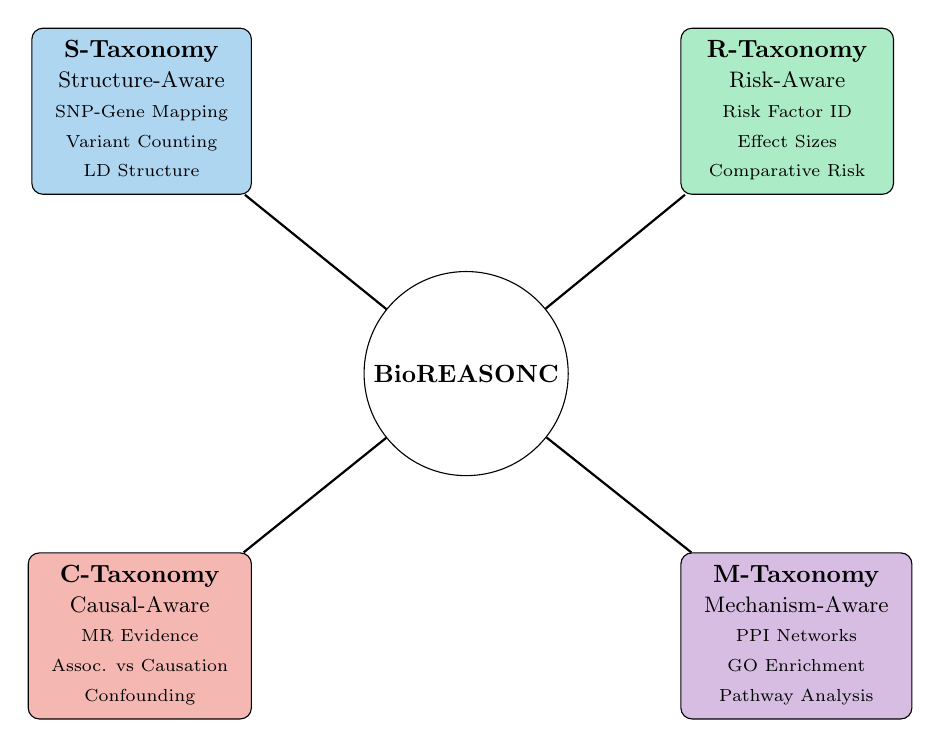
\begin{tikzpicture}[scale=0.9, transform shape]

% Central node
\node[circle, draw, fill=white, minimum size=2cm] (center) {\textbf{BioREASONC}};

% Taxonomy nodes
\node[rectangle, rounded corners, draw, fill=taxonomy_s!40, minimum width=3cm, minimum height=2cm, above left=1.5cm and 2cm of center] (S) {
    \begin{tabular}{c}
    \textbf{S-Taxonomy}\\
    \small Structure-Aware\\
    \scriptsize SNP-Gene Mapping\\
    \scriptsize Variant Counting\\
    \scriptsize LD Structure
    \end{tabular}
};

\node[rectangle, rounded corners, draw, fill=taxonomy_r!40, minimum width=3cm, minimum height=2cm, above right=1.5cm and 2cm of center] (R) {
    \begin{tabular}{c}
    \textbf{R-Taxonomy}\\
    \small Risk-Aware\\
    \scriptsize Risk Factor ID\\
    \scriptsize Effect Sizes\\
    \scriptsize Comparative Risk
    \end{tabular}
};

\node[rectangle, rounded corners, draw, fill=taxonomy_c!40, minimum width=3cm, minimum height=2cm, below left=1.5cm and 2cm of center] (C) {
    \begin{tabular}{c}
    \textbf{C-Taxonomy}\\
    \small Causal-Aware\\
    \scriptsize MR Evidence\\
    \scriptsize Assoc. vs Causation\\
    \scriptsize Confounding
    \end{tabular}
};

\node[rectangle, rounded corners, draw, fill=taxonomy_m!40, minimum width=3cm, minimum height=2cm, below right=1.5cm and 2cm of center] (M) {
    \begin{tabular}{c}
    \textbf{M-Taxonomy}\\
    \small Mechanism-Aware\\
    \scriptsize PPI Networks\\
    \scriptsize GO Enrichment\\
    \scriptsize Pathway Analysis
    \end{tabular}
};

% Arrows
\draw[thick] (center) -- (S);
\draw[thick] (center) -- (R);
\draw[thick] (center) -- (C);
\draw[thick] (center) -- (M);

\end{tikzpicture}
\caption{Four-Taxonomy Framework for Biomedical Reasoning Evaluation}
\label{fig:taxonomy}
\end{figure}

\subsubsection{Taxonomy Definitions}

\begin{description}
    \item[S-Taxonomy (Structure-Aware):] Evaluates understanding of genomic structure, including SNP-to-gene mapping, variant identification, and linkage disequilibrium patterns. Questions test factual recall and structural reasoning.

    \item[R-Taxonomy (Risk-Aware):] Assesses interpretation of genetic risk factors, including odds ratio interpretation, effect size comparison, and population-specific risk assessment.

    \item[C-Taxonomy (Causal-Aware):] The most critical taxonomy, testing the ability to distinguish association from causation using Mendelian Randomization evidence. This directly addresses the ``correlation does not imply causation'' principle.

    \item[M-Taxonomy (Mechanism-Aware):] Evaluates understanding of biological mechanisms through protein-protein interaction networks and Gene Ontology enrichment analysis.
\end{description}

\subsection{Answer Format Specification}

To comprehensively evaluate LLM capabilities, we implement five distinct answer formats for each question:

\begin{table}[htbp]
\centering
\caption{Five Answer Formats with Evaluation Criteria}
\label{tab:formats}
\begin{tabular}{p{2.5cm}p{4cm}p{5cm}}
\toprule
\textbf{Format} & \textbf{Description} & \textbf{Evaluation Metric} \\
\midrule
Yes/No & Binary classification with brief justification & Accuracy, F1-score \\
\addlinespace
Multiple Choice & Four options (A, B, C, D) with one correct & Accuracy, confusion matrix \\
\addlinespace
Short Answer & 1-2 sentence factual response & ROUGE, BERTScore, factual accuracy \\
\addlinespace
Long Answer & Detailed paragraph explanation & ROUGE, coherence, completeness \\
\addlinespace
Reasoning & Step-by-step logical reasoning & Chain-of-thought evaluation, logical consistency \\
\bottomrule
\end{tabular}
\end{table}

\subsection{Question Generation Pipeline}

Algorithm \ref{alg:generation} describes the benchmark generation process.

\begin{algorithm}[htbp]
\caption{Benchmark Generation Pipeline}
\label{alg:generation}
\begin{algorithmic}[1]
\Require Knowledge Graph $\mathcal{G}$, target size $n$, formats $\mathcal{F}$
\Ensure Benchmark dataset $\mathcal{B}$

\State $\mathcal{B} \gets \emptyset$
\State $\mathcal{P} \gets \text{SamplePairs}(\mathcal{G}, n, \text{stratify}=\text{evidence\_level})$

\For{each pair $p \in \mathcal{P}$}
    \For{each taxonomy $\tau \in \{S, R, C, M\}$}
        \State $\mathcal{T} \gets \text{GetTemplates}(\tau)$
        \For{each template $t \in \mathcal{T}$}
            \For{each format $f \in \mathcal{F}$}
                \State $q \gets \text{GenerateQuestion}(p, t, f)$
                \State $a \gets \text{GenerateAnswer}(p, t, f)$
                \State $\mathcal{B} \gets \mathcal{B} \cup \{(q, a, \tau, f, p)\}$
            \EndFor
        \EndFor
    \EndFor
\EndFor

\State \Comment{Add negative examples}
\State $\mathcal{W} \gets \text{GetWeakEvidencePairs}(\mathcal{G})$
\For{each $p \in \mathcal{W}$}
    \State Generate negative examples with ``No'' answers
\EndFor

\State \Return $\mathcal{B}$
\end{algorithmic}
\end{algorithm}

\subsection{Template-Based Question Generation}

Questions are generated using structured templates that ensure consistency and coverage:

\begin{lstlisting}[language=Python, caption=Template Structure Example, basicstyle=\small\ttfamily]
"R-RISK-FACTOR": {
    "taxonomy": "R",
    "category": "Risk Factor Identification",
    "formats": {
        "yes_no": {
            "question": "Is {gene} a genetic risk factor
                         for {disease}?",
            "answer_positive": "Yes. {gene} is a risk
                factor with {evidence_level} evidence.",
            "answer_negative": "No. {gene} shows weak
                evidence (score: {risk_score})."
        },
        "mcq": {
            "question": "What is the evidence level?",
            "options": {"A": "Very strong", "B": "Strong",
                       "C": "Moderate", "D": "Weak"}
        },
        ...
    }
}
\end{lstlisting}

\subsection{Evidence-Based Answer Generation}

Answers are generated based on the underlying evidence scores:

\begin{equation}
\text{Answer}(q, p) =
\begin{cases}
\text{Positive} & \text{if } S_{\text{evidence}}(p) > \theta_{\text{pos}} \\
\text{Negative} & \text{if } S_{\text{evidence}}(p) < \theta_{\text{neg}} \\
\text{Uncertain} & \text{otherwise}
\end{cases}
\end{equation}

For the C-taxonomy (causal questions), we specifically use MR scores:

\begin{equation}
\text{Causal\_Claim}(p) =
\begin{cases}
\text{Supported} & \text{if } S_{\text{MR}}(p) > 0.5 \\
\text{Suggestive} & \text{if } 0.3 < S_{\text{MR}}(p) \leq 0.5 \\
\text{Not Supported} & \text{if } S_{\text{MR}}(p) \leq 0.3
\end{cases}
\end{equation}

\subsection{Negative Example Generation}

To test the model's ability to correctly identify weak evidence and say ``No,'' we include negative examples:

\begin{itemize}
    \item \textbf{R-RISK-FACTOR-NEG}: Gene-disease pairs with risk\_score $< 0.3$
    \item \textbf{C-MR-EVIDENCE-NEG}: Pairs with MR\_score $< 0.2$ (no causal support)
    \item \textbf{M-PATHWAY-NEG}: Pairs with GO\_score $< 0.2$ (weak pathway connection)
\end{itemize}

\subsection{Multi-LLM Validation}

Generated questions and answers undergo validation using multiple LLMs to ensure quality:

\begin{figure}[htbp]
\centering
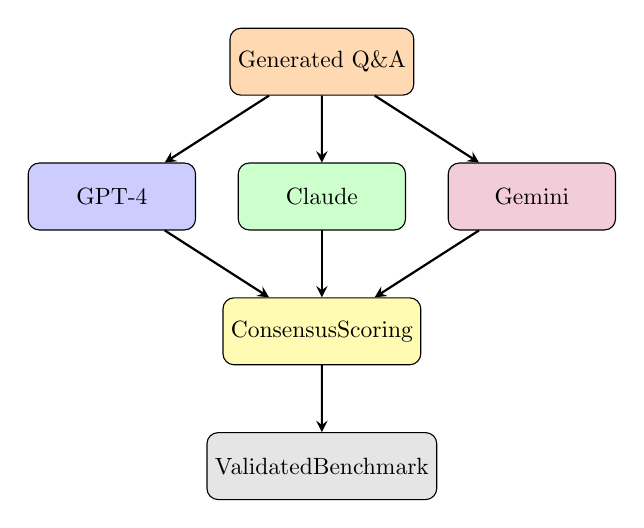
\begin{tikzpicture}[node distance=1cm, scale=0.85, transform shape]

\node[module, fill=orange!30] (input) {Generated Q\&A};

\node[module, below left=1cm and 0.5cm of input, fill=blue!20] (llm1) {GPT-4};
\node[module, below=1cm of input, fill=green!20] (llm2) {Claude};
\node[module, below right=1cm and 0.5cm of input, fill=purple!20] (llm3) {Gemini};

\node[module, below=1cm of llm2, fill=yellow!30] (consensus) {Consensus\\Scoring};

\node[module, below=1cm of consensus, fill=gray!20] (output) {Validated\\Benchmark};

\draw[arrow] (input) -- (llm1);
\draw[arrow] (input) -- (llm2);
\draw[arrow] (input) -- (llm3);
\draw[arrow] (llm1) -- (consensus);
\draw[arrow] (llm2) -- (consensus);
\draw[arrow] (llm3) -- (consensus);
\draw[arrow] (consensus) -- (output);

\end{tikzpicture}
\caption{Multi-LLM Validation Pipeline}
\label{fig:validation}
\end{figure}

The consensus score is computed as:

\begin{equation}
S_{\text{consensus}} = \frac{1}{|\mathcal{L}|} \sum_{l \in \mathcal{L}} S_l \cdot w_l
\end{equation}

where $\mathcal{L}$ is the set of validator LLMs and $w_l$ are reliability weights.

%==============================================================================
\section{Implementation Details}
%==============================================================================

\subsection{Data Classes}

\begin{lstlisting}[language=Python, caption=Core Data Structures, basicstyle=\small\ttfamily]
@dataclass
class GeneDiseasePair:
    gene_name: str
    disease_name: str
    risk_weight_score: float      # GWAS evidence
    causal_confidence_score: float # Fine-mapping
    mr_score: float               # MR validation
    go_functional_score: float    # Pathway evidence
    snp_count: int                # Supporting variants
    evidence_level: EvidenceLevel

@dataclass
class KGGeneratedItem:
    id: str
    taxonomy: str                 # S, R, C, or M
    question: str
    answer: str
    answer_format: str            # yes_no, mcq, etc.
    ground_truth: Dict[str, Any]
    difficulty: str
    evidence_level: str
\end{lstlisting}

\subsection{Scaling Strategy}

Table \ref{tab:scaling} presents the controlled scaling strategy per taxonomy.

\begin{table}[htbp]
\centering
\caption{Dataset Scaling Strategy}
\label{tab:scaling}
\begin{tabular}{lcccc}
\toprule
\textbf{Taxonomy} & \textbf{Small} & \textbf{Medium} & \textbf{Large} & \textbf{Full} \\
\midrule
S (Structure) & 100 & 500 & 2,000 & 10,000 \\
R (Risk) & 100 & 500 & 2,000 & 10,000 \\
C (Causal) & 100 & 500 & 2,000 & 10,000 \\
M (Mechanism) & 100 & 500 & 2,000 & 10,000 \\
\midrule
\textbf{Total} & 400 & 2,000 & 8,000 & 40,000 \\
$\times$ 5 formats & 2,000 & 10,000 & 40,000 & 200,000 \\
\bottomrule
\end{tabular}
\end{table}

%==============================================================================
\section{Evaluation Metrics}
%==============================================================================

\subsection{Format-Specific Metrics}

\begin{description}
    \item[Yes/No Questions:] Accuracy, Precision, Recall, F1-Score
    \item[Multiple Choice:] Accuracy, Per-option analysis
    \item[Short/Long Answers:] ROUGE-L, BERTScore, Factual Accuracy
    \item[Reasoning:] Chain-of-thought coherence, Logical validity
\end{description}

\subsection{Taxonomy-Specific Evaluation}

\begin{equation}
\text{Score}_{\tau} = \alpha \cdot \text{Accuracy}_{\tau} + \beta \cdot \text{Reasoning}_{\tau} + \gamma \cdot \text{Faithfulness}_{\tau}
\end{equation}

For C-taxonomy (causal), we specifically measure:
\begin{itemize}
    \item \textbf{Overclaim Rate}: Frequency of claiming causation without MR evidence
    \item \textbf{Underclaim Rate}: Failure to recognize MR-validated causal relationships
    \item \textbf{Causal Precision}: Correct causal claims / Total causal claims
\end{itemize}

%==============================================================================
\section{Conclusion}
%==============================================================================

BioREASONC-Bench provides a rigorous framework for evaluating LLM causal reasoning in biomedicine. Key contributions include:

\begin{enumerate}
    \item A four-taxonomy framework covering structure, risk, causal, and mechanism reasoning
    \item Five answer formats enabling comprehensive capability assessment
    \item Integration with MR-validated evidence for ground-truth causal relationships
    \item Negative examples testing the ability to recognize weak evidence
    \item Multi-LLM validation ensuring benchmark quality
\end{enumerate}

The benchmark is designed to identify specific weaknesses in LLM reasoning, particularly the critical distinction between genetic association and causation---a distinction with significant implications for clinical decision-making and drug target identification.

%==============================================================================
% References
%==============================================================================
\begin{thebibliography}{9}

\bibitem{causaldb2}
Wang, J., et al. (2023). CAUSALdb2: An updated database for causal variants and genes of complex traits. \textit{Nucleic Acids Research}.

\bibitem{mr}
Davey Smith, G., \& Hemani, G. (2014). Mendelian randomization: genetic anchors for causal inference. \textit{Human Molecular Genetics}.

\bibitem{gwas}
Buniello, A., et al. (2019). The NHGRI-EBI GWAS Catalog. \textit{Nucleic Acids Research}.

\end{thebibliography}

\end{document}
